% grut_architecture.tex — Figure 1 of the GRUT public record.
% Build: xelatex grut_architecture.tex  (standalone; produces grut_architecture.pdf)
\documentclass[border=6pt]{standalone}
\usepackage{fontspec}
\setmainfont{Latin Modern Roman}
\usepackage{unicode-math}
\setmathfont{Latin Modern Math}
\usepackage{tikz}
\usetikzlibrary{positioning,arrows.meta,fit,backgrounds,calc}
\definecolor{core}{RGB}{214,234,216}      % derived in class
\definecolor{cond}{RGB}{252,228,196}      % conditional branch
\definecolor{supp}{RGB}{230,230,230}      % supplied inputs
\definecolor{acc}{RGB}{210,224,245}       % access (cross-cutting)
\definecolor{seam}{RGB}{190,40,40}
\begin{document}
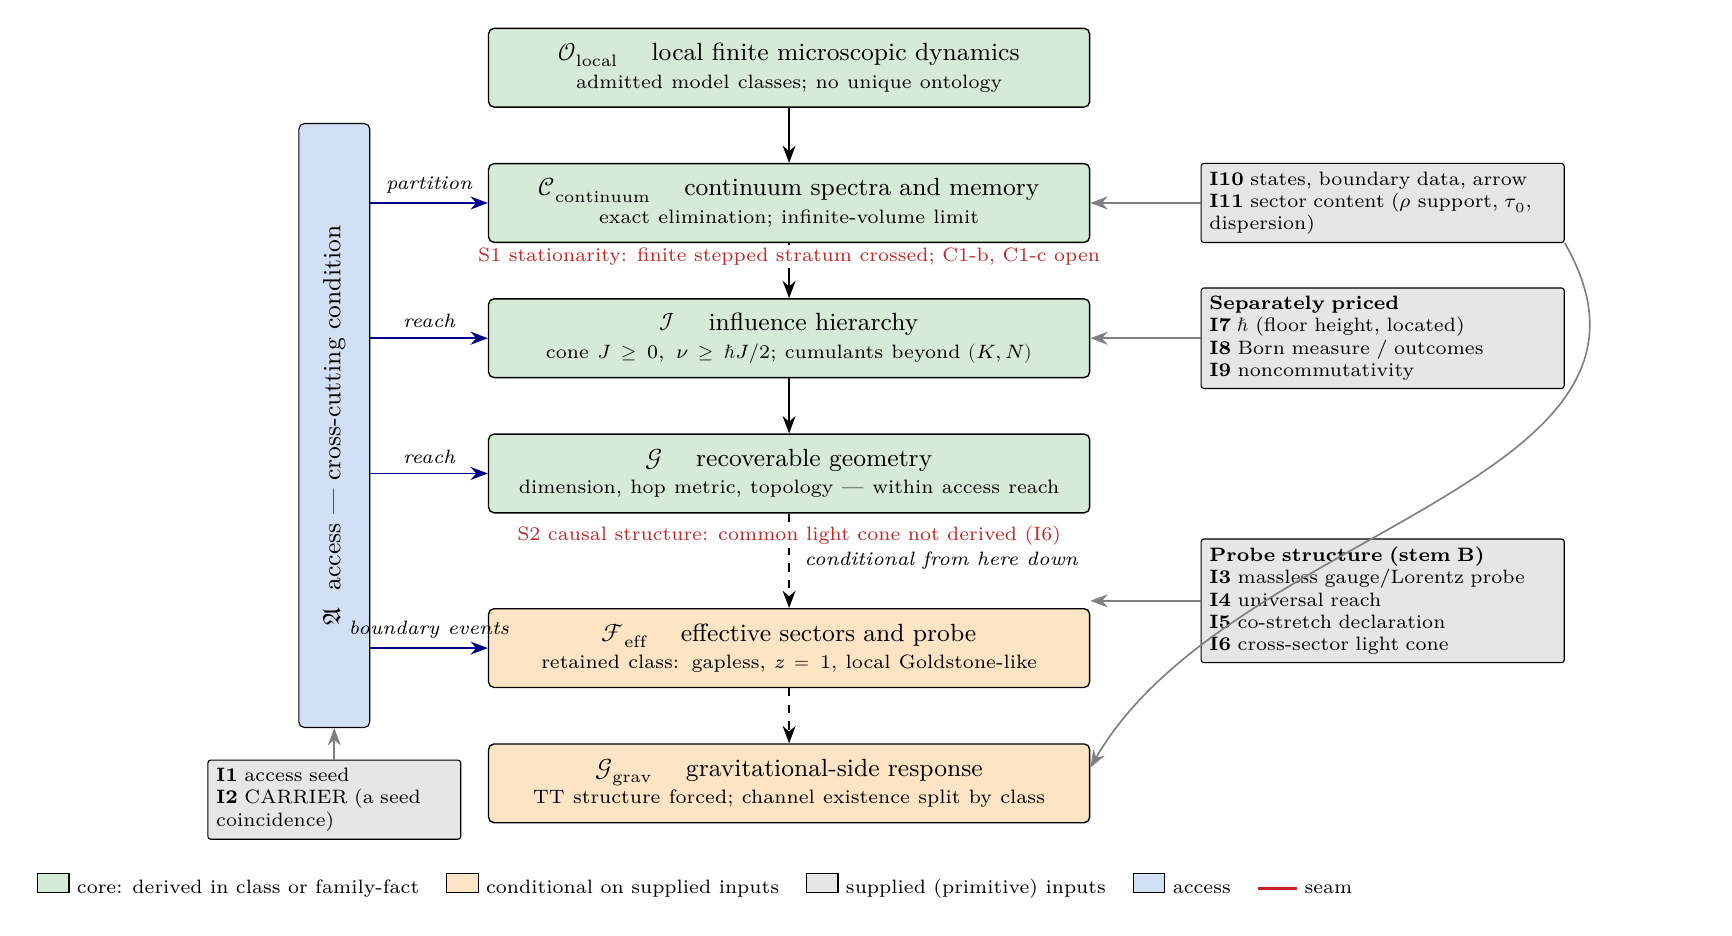
\begin{tikzpicture}[
  node distance=7mm and 10mm,
  layer/.style={draw, rounded corners=2pt, text width=74mm, minimum height=10mm,
                align=center, font=\small, line width=0.5pt},
  inp/.style={draw, rounded corners=1pt, fill=supp, font=\scriptsize, align=left,
              inner sep=3pt, text width=44mm},
  arr/.style={-{Stealth[length=2.2mm]}, line width=0.6pt},
  lbl/.style={font=\scriptsize\itshape, align=left},
]
% --- the chain ---
\node[layer, fill=core] (O) {$\mathcal O_{\rm local}$ \quad local finite microscopic dynamics\\[-1pt]
  {\scriptsize admitted model classes; no unique ontology}};
\node[layer, fill=core, below=of O] (C) {$\mathcal C_{\rm continuum}$ \quad continuum spectra and memory\\[-1pt]
  {\scriptsize exact elimination; infinite-volume limit}};
\node[layer, fill=core, below=of C] (I) {$\mathcal I$ \quad influence hierarchy\\[-1pt]
  {\scriptsize cone $J\ge0,\ \nu\ge\hbar J/2$; cumulants beyond $(K,N)$}};
\node[layer, fill=core, below=of I] (G) {$\mathcal G$ \quad recoverable geometry\\[-1pt]
  {\scriptsize dimension, hop metric, topology --- within access reach}};
\node[layer, fill=cond, below=12mm of G] (F) {$\mathcal F_{\rm eff}$ \quad effective sectors and probe\\[-1pt]
  {\scriptsize retained class: gapless, $z=1$, local Goldstone-like}};
\node[layer, fill=cond, below=of F] (GG) {$\mathcal G_{\rm grav}$ \quad gravitational-side response\\[-1pt]
  {\scriptsize TT structure forced; channel existence split by class}};

\draw[arr] (O) -- (C);
\draw[arr] (C) -- (I);
\draw[arr] (I) -- (G);
\draw[arr, dashed] (G) -- node[right, lbl, xshift=2pt] {conditional from here down} (F);
\draw[arr, dashed] (F) -- (GG);

% --- access bar (cross-cutting), to the left of the chain ---
\coordinate (atop) at ($(C.north west)+(-24mm,5mm)$);
\coordinate (abot) at ($(F.south west)+(-15mm,-5mm)$);
\node[draw, fill=acc, rounded corners=2pt, fit=(atop)(abot), inner sep=0pt] (A) {};
\node[rotate=90, font=\small] at (A.center) {$\mathfrak A$ \ access --- cross-cutting condition};
\draw[arr, draw=blue!55!black] (A.east |- C.west) -- node[above, lbl] {partition} (C.west);
\draw[arr, draw=blue!55!black] (A.east |- I.west) -- node[above, lbl] {reach} (I.west);
\draw[arr, draw=blue!55!black] (A.east |- G.west) -- node[above, lbl] {reach} (G.west);
\draw[arr, draw=blue!55!black] (A.east |- F.west) -- node[above, lbl] {boundary events} (F.west);
\node[inp, text width=30mm, below=4mm of A.south, anchor=north] (I1) {\textbf{I1} access seed\\\textbf{I2} CARRIER (a seed coincidence)};
\draw[arr, draw=gray] (I1.north) -- (A.south);

% --- supplied inputs entering the conditional branch ---
\node[inp, right=14mm of F, yshift=6mm] (Ib) {\textbf{Probe structure (stem B)}\\
  \textbf{I3} massless gauge/Lorentz probe\\ \textbf{I4} universal reach\\
  \textbf{I5} co-stretch declaration\\ \textbf{I6} cross-sector light cone};
\draw[arr, draw=gray] (Ib.west) -- (F.east |- Ib.west);
\node[inp, right=14mm of I] (Iq) {\textbf{Separately priced}\\
  \textbf{I7} $\hbar$ (floor height, located)\\ \textbf{I8} Born measure / outcomes\\
  \textbf{I9} noncommutativity};
\draw[arr, draw=gray] (Iq.west) -- (I.east);
\node[inp, right=14mm of C] (Ic) {\textbf{I10} states, boundary data, arrow\\
  \textbf{I11} sector content ($\rho$ support, $\tau_0$, dispersion)};
\draw[arr, draw=gray] (Ic.west) -- (C.east);
\draw[arr, draw=gray] (Ic.south east) to[out=-60,in=60] ($(GG.east)+(0,2mm)$);

% --- seams ---
\draw[seam, line width=1pt] ($(C.south west)+(4mm,-1.2mm)$) -- ($(C.south east)+(-4mm,-1.2mm)$);
\node[font=\scriptsize, text=seam, align=center, below=0.2mm of C.south, fill=white, inner sep=1pt]
  {S1 stationarity: finite stepped stratum crossed; C1-b, C1-c open};
\draw[seam, line width=1pt] ($(G.south west)+(4mm,-2mm)$) -- ($(G.south east)+(-4mm,-2mm)$);
\node[font=\scriptsize, text=seam, align=center, below=1.2mm of G.south, fill=white, inner sep=1pt]
  {S2 causal structure: common light cone not derived (I6)};

% --- legend ---
\node[below=5mm of GG, xshift=-12mm, font=\scriptsize, align=left] (L) {
  \tikz\node[fill=core,draw,minimum width=4mm,minimum height=2.5mm]{}; core: derived in class or family-fact \quad
  \tikz\node[fill=cond,draw,minimum width=4mm,minimum height=2.5mm]{}; conditional on supplied inputs \quad
  \tikz\node[fill=supp,draw,minimum width=4mm,minimum height=2.5mm]{}; supplied (primitive) inputs \quad
  \tikz\node[fill=acc,draw,minimum width=4mm,minimum height=2.5mm]{}; access \quad
  {\color{seam}\rule[0.4ex]{5mm}{1pt}} seam};
\end{tikzpicture}
\end{document}
